\begin{enumerate}[\Large\bfseries 1.]

%--------------------1.
\item \textbf{\large APLICACIÓN DE INTEGRALES}\\\\

    \begin{enumerate}[\bfseries a)]

	%----------a.
	\item \textbf{\large Tom Apostol, Calculus I, Capítulo 2, Problema 28}\\\\
	Demostrar las siguientes fórmulas de integración, válidas para $b\neq 0$.
	$$\int_0^x cos(a+bt)\; dt = \dfrac{1}{b}\left[\sen(a+bx)+\sen a\right],$$
	$$\int_0^x \sen (a+bt)\; dt = -\dfrac{1}{b} \left[\cos(a+bx)-\cos a\right].$$\\\\

	Demostración.-\; Usando la formula de adición tenemos,

	$$\begin{array}{rcl}
	    \displaystyle\int_0^x \cos(a+bt)\; dt&=&\displaystyle\int_0^x \left[\sen a \cos(bt)+\sen(bt)\cos a\right]\, dt\\\\
						 &=&\dfrac{\cos a}{b} \displaystyle\int_0^{bx} \cos t \; dt  - \dfrac{\sen a}{b} \displaystyle\int_0^{bx} \sen t \; dt \qquad b\neq 0\\\\
						 &=&\dfrac{1}{b}\left[\cos a \sen(bx)-\sen a + \sen a \cos(bx)\right]\\\\
						 &=&\dfrac{1}{b}\left[\sen(a+bx)-\sen a\right]\\\\

	\end{array}$$
	Similar a la anterior demostración tenemos, \\

	 $$\begin{array}{rcl}
	     \displaystyle\int_0^x \sen(a+bt)\; dt&=&\displaystyle\int_0^x \left[\sen a \cos(bt)+\sen(bt)\cos a\right]\; dt\\\\
						  &=&\dfrac{\sen a}{b} \displaystyle\int_0^{bx} \cos t \; dt - \dfrac{\cos a}{b}\int_0^{bx} \sen t \; dt \qquad b\neq 0\\\\
						  &=&\dfrac{\sen a}{b}\sen(bx)+\dfrac{\cos a}{b}(1-\cos(bx))\\\\
						  &=&\dfrac{1}{b}\left[\sen a \sen (bx) + \cos a - \cos a \cos (bx)\right]\\\\
						  &=&-\dfrac{1}{b} \left[\cos(a+bx)-\cos a\right]\\\\
	 \end{array}$$

	%----------b)
	\item \textbf{Código fuente.}\\ 
	    
	    \lstinputlisting[language=Python]{python/tareas_mat/week6/py1.py}
	    \vspace{.5cm}
	
	%----------c)
	\item \textbf{Prueba de la ejecución del programa}.\\
	    \begin{center}
		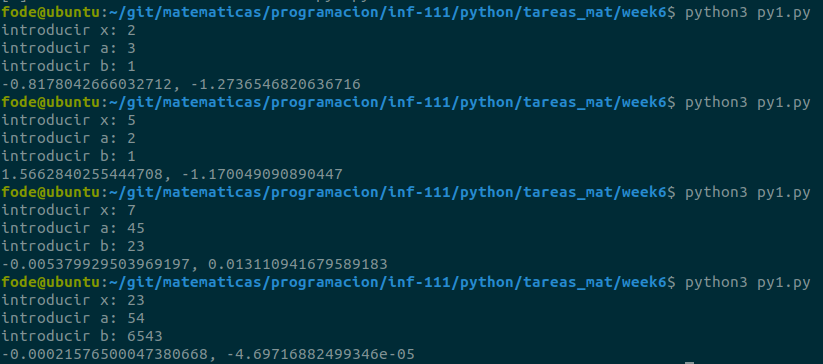
\includegraphics[scale=.55]{imagenes/tareas_mat/week6/py1.png}
	    \end{center}

    \end{enumerate}

\newpage

%--------------------2.
\item \textbf{\large APLICACIÓN DE INTEGRALES}\\\\

    \begin{enumerate}[\bfseries a)]

	%----------a.
	\item \textbf{\large Tom Apostol, Calculus I, Capítulo 2, Problema 21}\\\\
	$\displaystyle\int_0^{\pi/2} |\sen x - \cos x|\; dx$\\\\
	Respuesta.-\; Ya que $\cos x - \sen x \geq 0$ esta definida por $\left(0,\frac{\pi}{4}\right)$ y $\cos x - \sen x < 0$ esta dado por $\left(\frac{\pi}{4},\frac{\pi}{2}\right]$ tenemos,
	\begin{center}
	    \begin{tabular}{rcl}
		$\displaystyle\int_0^{\pi/2} |\sen x - \cos x|\; dx$&$=$&$\displaystyle\int_0^{\pi/4}(\cos x - \sen x)\; dx + \int_{\pi/4}^{\pi/2}(\sen x - \cos x)\; dx$\\\\
								    &$=$&$\sen\left(\dfrac{\pi}{4}\right)-\left[1-\cos\left(\dfrac{\pi}{4}\right)\right]  -\left[\cos\left(\dfrac{\pi}{2}\right)-\cos\left(\dfrac{\pi}{4}\right)\right]+\left[\sen\left(\dfrac{\pi}{2}\right)-\sen \left(\dfrac{\pi}{4}\right)\right]$\\\\
								    &$=$&$\dfrac{\sqrt{2}}{2}+\dfrac{\sqrt{2}}{2}-1+\dfrac{\sqrt{2}}{2}-0-1+\dfrac{\sqrt{2}}{2}$\\\\
		  &$=$&$2\sqrt{2}-2$\\\\
	      \end{tabular}

	\end{center}

	%----------b)
	\item \textbf{Código fuente.}\\ 
	    
	    \lstinputlisting[language=Python]{python/tareas_mat/week6/py21.py}
	    \vspace{.5cm}
	
	%----------c)
	\item \textbf{Prueba de la ejecución del programa}.\\
	    \begin{center}
		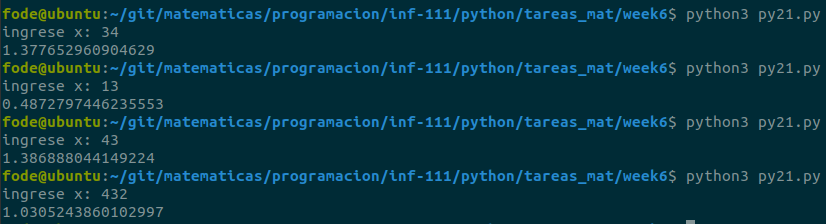
\includegraphics[scale=.55]{imagenes/tareas_mat/week6/py21.png}
	    \end{center}

    \end{enumerate}

\newpage

%--------------------3.
\item \textbf{\large APLICACIÓN DE INTEGRALES}\\\\

    \begin{enumerate}[\bfseries a)]

	%----------a.
	\item \textbf{\large Tom Apostol, Calculus I, Capítulo 2, Problema 23}\\\\
	$\displaystyle\int_0^\pi  \bigg|\dfrac{1}{2} + \cos t\bigg|\; dx$.\\\\
	    \begin{center}
		\begin{tabular}{rcl}
		    $\displaystyle\int_{0}^{\pi} \bigg| \dfrac{1}{2}+\cos t\bigg| \; dt$&$=$&$\displaystyle\int_0^{\frac{2\pi}{3}}\left(\dfrac{1}{2} + \cos t\right)\; dt + \int_{\frac{2\pi}{3}}^{\pi}\left(\dfrac{1}{2} + \cos t\right)\; dt$\\\\
											&$=$&$\displaystyle\int_0^{\frac{2\pi}{3}} \dfrac{1}{2}\; dt + \int_{0}^{\frac{2\pi}{3}} \cos(t) \; dt - \int_{\frac{2\pi}{3}}\pi \dfrac{1}{2}\; dt + \int_{\frac{2\pi}{3}}^\pi \cos(t) \; dt$\\\\
											&$=$&$\dfrac{t}{2}\bigg|_0^{\frac{2\pi}{3}} + \sen(t)\bigg|_{0}^{\frac{2\pi}{3}} -  \dfrac{t}{2} \bigg|_{\frac{2\pi}{3}}^\pi \dfrac{1}{2}\; dt - \sen(t)\bigg|_{\frac{2\pi}{3}}^\pi$\\\\
											&$=$&$\dfrac{\pi}{3}+\sen\left(\dfrac{2\pi}{3}\right) - \left(\dfrac{\pi}{2}-\dfrac{2\pi}{6}\right)-\left[\sen \pi - \sen\left( \dfrac{2\pi}{3}\right)\right]$\\\\
											&$=$&$\dfrac{\pi}{6}+\sqrt{3}$\\\\
		\end{tabular}
	    \end{center}

	%----------b)
	\item \textbf{Código fuente.}\\ 
	    
	    \lstinputlisting[language=Python]{python/tareas_mat/week6/py23.py}
	    \vspace{.5cm}
	
	%----------c)
	\item \textbf{Prueba de la ejecución del programa}.\\
	    \begin{center}
		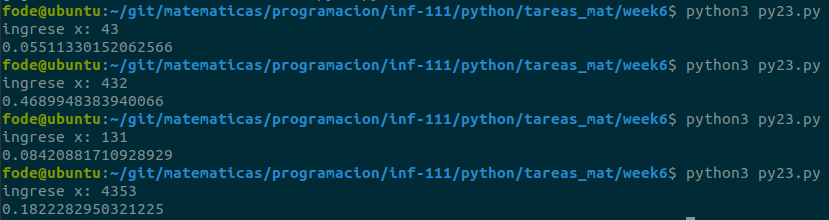
\includegraphics[scale=.55]{imagenes/tareas_mat/week6/py23.png}
	    \end{center}

    \end{enumerate}

\newpage

%--------------------4.
\item \textbf{\large APLICACIÓN DE INTEGRALES}\\\\

    \begin{enumerate}[\bfseries a)]

	%----------a.
	\item \textbf{\large Tom Apostol, Calculus I, Capítulo 2, Problema 29 (a)}\\\\
	Hacer uso de la identidad $\sen 3t = 3 \sen t  - 4 \sen^3 t$ para deducir la fórmula de integración
	    $$\int_0^x \sen^3 t \;dt = \frac{2}{3} - \frac{1}{3}(2\sen^2x)\cos x.$$

	    Respuesta.-\; $\sen^3 = \dfrac{3}{4} = \dfrac{3}{4}\sen t - \dfrac{1}{4}\sen(3t)$
	    $$ \begin{array}{rcl}
		\displaystyle\int_0^x \sen^3 t \; dx&=&\displaystyle \int_0^x\left[\dfrac{3}{4}\sen t - \dfrac{1}{4}\sen (3t)\right]\; dt\\\\
						    &=&\dfrac{3}{4}(1-\cos x)-\dfrac{1}{12}\displaystyle \int_0^x \sen t \; dt\\\\
						    &=&\dfrac{3}{4} - \dfrac{3}{4}\cos x - \dfrac{1}{12}+\dfrac{1}{12} \cos 3x\\\\
						    &=&\dfrac{2}{3}-\dfrac{3}{4}\cos x + \dfrac{1}{12}\left(\cos x  - 4\sen^2 x \cos x\right)\\\\
						    &=&\dfrac{2}{3}-\dfrac{2}{3}\cos x - \dfrac{1}{2}\sen^2 x \cos x\\\\
						    &=&\dfrac{2}{3}-\dfrac{1}{3}\left(2+\sen^2 x\right)\cos x\\\\
	    \end{array}$$

	%----------b)
	\item \textbf{Código fuente.}\\ 
	    
	    \lstinputlisting[language=Python]{python/tareas_mat/week6/py29a.py}
	    \vspace{.5cm}
	
	%----------c)
	\item \textbf{Prueba de la ejecución del programa}.\\
	    \begin{center}
		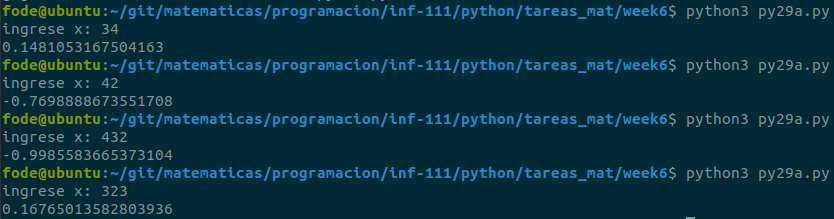
\includegraphics[scale=.55]{imagenes/tareas_mat/week6/py29a.png}
	    \end{center}

    \end{enumerate}

\newpage


%--------------------5.
\item \textbf{\large APLICACIÓN DE INTEGRALES}\\\\

    \begin{enumerate}[\bfseries a)]

	%----------a.
	\item \textbf{\large Tom Apostol, Calculus I, Capítulo 2, Problema 29 (b)}\\\\
	Deducir la identidad $\cos 3t = 4\cos^3 t - 3\cos t$ y utilizándola para demostrar que 
	    $$\int_0^x \cos^3 t \; dt = \frac{1}{3}(2+\cos^2 x)\sen x$$
	    Respuesta.-\; $\cos3 x = 4\cos^2 - 3\cos x$

	    $$\begin{array}{rcl}
		\displaystyle\int_0^x \cos^3 t\; dt&=&\displaystyle\int_0^x \left[\cos(3t) + 3\cos t\right]\; dt\\\\
						   &=&\dfrac{1}{4}\displaystyle\int_0^x \cos(3t)\; dt + \displaystyle\int_0^x \cos t \; dt\\\\
						   &=&\dfrac{1}{12}\displaystyle\int_0^3x \cos t \; dt + \dfrac{3}{4}\displaystyle\int_0^x \cos t \; dt\\\\
						   &=&\dfrac{1}{12} \sen(3t) \; dt + \dfrac{3}{4}\sen x\\\\
						   &=&\dfrac{1}{12}(3\sen x - 4 \sen^3 x) + \dfrac{3}{4}\sen x\\\\
						   &=&\sen x \dfrac{1}{3}\sen^3 x\\\\
						   &=&\sen x \dfrac{1}{3}\sen^2x \sen x\\\\
						   &=&\sen x - \dfrac{1}{3}\sen^2x \sen x\\\\
						   &=&\left[1 - \dfrac{1}{3}\left(1-\cos^2 x\right)\right]\sen x\\\\
						   &=&\left(\dfrac{2}{3}+\dfrac{1}{3}\cos^2 x\right)\sen x\\\\
						   &=&\dfrac{1}{3}\left(2+\cos^2 x\right)\sen x\\\\
		\end{array}$$

	%----------b)
	\item \textbf{Código fuente.}\\ 
	    
	    \lstinputlisting[language=Python]{python/tareas_mat/week6/py29b.py}
	    \vspace{1cm}
	
	%----------c)
	\item \textbf{Prueba de la ejecución del programa}.\\
	    \begin{center}
		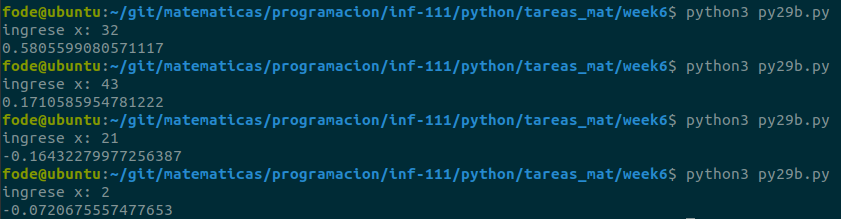
\includegraphics[scale=.55]{imagenes/tareas_mat/week6/py29b.png}
	    \end{center}

    \end{enumerate}

\newpage

\end{enumerate}
